\documentclass[11pt,a4paper]{article}
\usepackage[utf8]{inputenc}
\usepackage{geometry}
\usepackage{graphicx}
\usepackage{tikz}
\usepackage{hyperref}
\usepackage{xcolor}
\usepackage{listings}
\usepackage{float}
\usetikzlibrary{shapes.geometric, arrows, positioning, calc, backgrounds, fit}

\geometry{margin=1in}

% Brand Colors
\definecolor{basaltDark}{HTML}{0A0A0A}
\definecolor{basaltAccent}{HTML}{6B7280}
\definecolor{basaltHighlight}{HTML}{3B82F6}

% TIKZ Styles
\tikzstyle{process} = [rectangle, minimum width=3cm, minimum height=1cm, text centered, draw=black, fill=white]
\tikzstyle{decision} = [diamond, minimum width=3cm, minimum height=1cm, text centered, draw=black, fill=white]
\tikzstyle{arrow} = [thick,->,>=stealth]
\tikzstyle{cloud} = [draw, ellipse, fill=gray!20, minimum height=2em]
\tikzstyle{nodebox} = [rectangle, rounded corners, minimum width=3cm, minimum height=1.5cm, text centered, draw=basaltDark, fill=basaltHighlight!10]

\title{\textbf{BasaltSurge Decentralization Proposal} \\ \large Transitioning to a Sovereign, Hybrid Node Architecture}
\author{BasaltSurge Planning Team}
\date{\today}

\begin{document}

\maketitle
\tableofcontents
\newpage

\section{Executive Summary}
BasaltSurge is transitioning from a partner-container model to a fully decentralized \textbf{Node} architecture. This shift allows for infinite scalability, 100\% uptime via redundancy, and true data sovereignty for merchants. 

The new architecture introduces:
\begin{itemize}
    \item \textbf{Decentralized Nodes}: Independent operators hosting compute instances.
    \item \textbf{Basalt Distributed Storage (BDS)}: A gasless, peer-to-peer storage mesh for shop data.
    \item \textbf{Dynamic Incentives}: A 0.20\% fee share for Node Providers.
    \item \textbf{Automatic Split Deployment}: "Invisible" smart contract deployment sponsored by the platform.
\end{itemize}

\section{System Architecture}

\subsection{Hybrid Routing Model}
While the execution is decentralized, the entry point remains unified to ensure trust and ease of use. A Global Edge Router directs traffic to the optimal Node based on geography and health.

\begin{figure}[H]
\centering
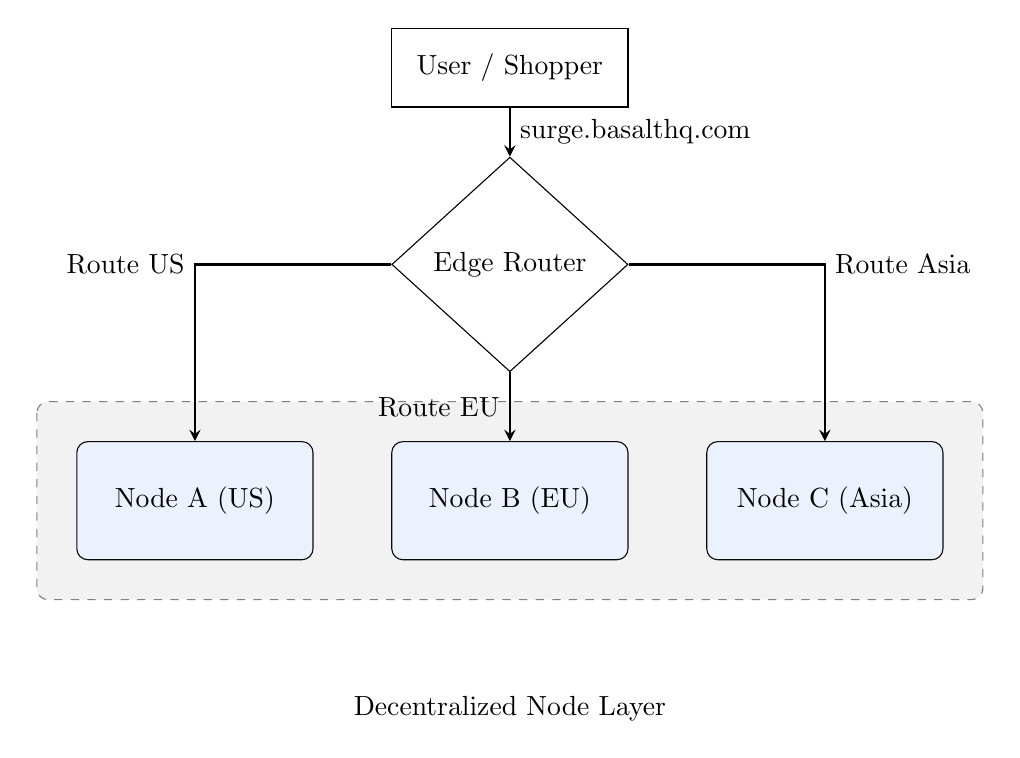
\begin{tikzpicture}[node distance=2cm]

% Nodes
\node (user) [process] {User / Shopper};
\node (edge) [decision, below of=user, yshift=-0.5cm] {Edge Router};
\node (nodeA) [nodebox, below of=edge, xshift=-4cm, yshift=-1cm] {Node A (US)};
\node (nodeB) [nodebox, below of=edge, yshift=-1cm] {Node B (EU)};
\node (nodeC) [nodebox, below of=edge, xshift=4cm, yshift=-1cm] {Node C (Asia)};

% Links
\draw [arrow] (user) -- node[anchor=west] {surge.basalthq.com} (edge);
\draw [arrow] (edge) -| node[anchor=east, pos=0.5] {Route US} (nodeA);
\draw [arrow] (edge) -- node[anchor=east] {Route EU} (nodeB);
\draw [arrow] (edge) -| node[anchor=west, pos=0.5] {Route Asia} (nodeC);

% Backgrounds
\begin{pgfonlayer}{background}
    \path (nodeA.west |- nodeA.north)+(-0.5,0.5) node (a) {};
    \path (nodeC.east |- nodeC.south)+(0.5,-0.5) node (b) {};
    \path[fill=gray!10,rounded corners, draw=black!50, dashed] (a) rectangle (b);
    \node [below=0.1cm of nodeB, yshift=-1.5cm] {Decentralized Node Layer};
\end{pgfonlayer}

\end{tikzpicture}
\caption{Hybrid Routing Architecture}
\end{figure}

\section{Basalt Distributed Storage (BDS)}

To achieve true resilience, we must decouple \textit{Compute} from \textit{Data}. BDS is a custom gossip protocol where nodes replicate specialized "Vaults" of merchant data.

\subsection{Storage Protocol}
\begin{enumerate}
    \item \textbf{The Vault}: A cryptographically signed append-only log of JSON documents (Inventory, Config).
    \item \textbf{The Swarm}: A mesh of nodes that replicate Vaults.
    \item \textbf{Persistence}: Data is stored on Docker Volumes, surviving container restarts.
\end{enumerate}

\begin{figure}[H]
\centering
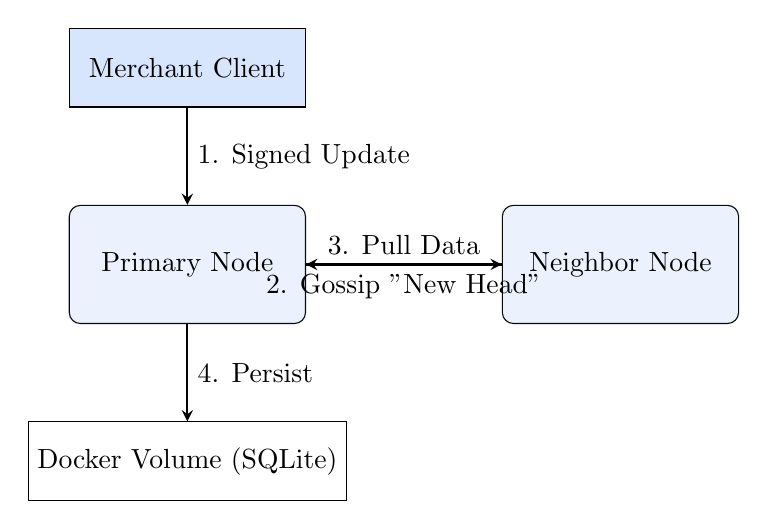
\begin{tikzpicture}[node distance=2.5cm]

\node (merchant) [process, fill=basaltHighlight!20] {Merchant Client};
\node (primary) [nodebox, below of=merchant] {Primary Node};
\node (neighbor) [nodebox, right of=primary, xshift=3cm] {Neighbor Node};
\node (db) [process, below of=primary] {Docker Volume (SQLite)};

\draw [arrow] (merchant) -- node[anchor=west] {1. Signed Update} (primary);
\draw [arrow] (primary) -- node[anchor=north] {2. Gossip "New Head"} (neighbor);
\draw [arrow] (neighbor) -- node[anchor=south] {3. Pull Data} (primary);
\draw [arrow] (primary) -- node[anchor=west] {4. Persist} (db);

\end{tikzpicture}
\caption{BDS Replication Flow}
\end{figure}

\section{Operational Model}

\subsection{Node Registration}
Nodes register on-chain via the \textbf{Basalt Diamond Proxy}. This acts as both the registry and the Global Loyalty Pool wallet.
\begin{itemize}
    \item \textbf{Platform}: BasaltSurge
    \item \textbf{Registry}: Diamond Contract
    \item \textbf{Requirement}: Proof of active Endpoint
\end{itemize}

\subsection{Gasless Operations}
Node operators do not need ETH for operations. 
\begin{itemize}
    \item \textbf{Signing}: Nodes use a private key to sign \textit{intent} (e.g., "Deploy Split").
    \item \textbf{Sponsorship}: The Platform's Relayer submits the transaction and pays the gas.
\end{itemize}

\section{Economic Model}

The migration introduces a 4-way fee split to align incentives across the network.

\begin{table}[H]
\centering
\begin{tabular}{|l|l|l|}
\hline
\textbf{Stakeholder} & \textbf{Share} & \textbf{Purpose} \\ \hline
Merchant & 99.50\% & Net Revenue \\ \hline
Platform & 0.25\% & Governance \& Development \\ \hline
Node Provider & 0.20\% & Infrastructure Incentive \\ \hline
Loyalty Pool & 0.05\% & Community Rewards (Global) \\ \hline
\end{tabular}
\caption{Transaction Fee Distribution}
\end{table}

\section{Implementation Roadmap}

\begin{itemize}
    \item \textbf{Phase 1: Hybrid Core} (Current)
    \begin{itemize}
        \item Implement Environment Config for \texttt{NODE\_PRIVATE\_KEY}.
        \item Deploy Diamond Proxy for Registry.
    \end{itemize}
    
    \item \textbf{Phase 2: BDS Integration}
    \begin{itemize}
        \item Build "Vault" logic for signed updates.
        \item Implement Docker Volume persistence.
    \end{itemize}
    
    \item \textbf{Phase 3: Public Beta}
    \begin{itemize}
        \item Check \texttt{install\_node.sh} script.
        \item Onboard first external Node Providers.
    \end{itemize}
\end{itemize}

\section{Conclusion}
This proposal outlines a path to a robust, uncensorable commerce network. By leveraging a hybrid routing model and the custom Basalt Distributed Storage protocol, we ensure speed, reliability, and true sovereignty for all participants.

\end{document}
